\section{Yeast Data}\label{sec:data}

% Here we will introduce our data sources and how we process them.

\subsection{Data Describtion}

We explored the effects of different statistical methods by by the analysis of a yeast eQTL data set described by \citet{brem2005landscape}, where $n = 112$ segregants were grown from a cross between two budding yeast strains, BY4716 and RM11-1a. 
For each of the segregants, gene expression was profiled on microarrays containing $6216$ genes, and genotyping was performed at $2957$ markers. 

Genotype is a categorical variables with a value of $0$ or $1$, and gene expression level is given by $log2(\text{sample}/\text{BY reference})$. 

\subsection{Data Preparation}

\subsubsection{Processing Markers Data}

The DNA of the same organism has a very high similarity. 
For example, all humans are $99.9\%$ identical and, of that tiny $0.1\%$ difference. 
Considering the similarity of markers, we found that different markers in the data may have identical or differ at most few yeast samples after exploratory data analysis. 

Inspired by \citet{yin2011sparse}, we combined the markers into $949$ blocks such that markers with the same block differed by at most one sample, and one representative marker was chosen from each block. 
To accomplish that, we used hierarchical clustering with complete-linkage criteria and cut the clustering tree at distance $d=1$. 
Note that the value of the marker data is only 0 or 1, so we can use any distance function, like Euclidean distance or Manhattan distance, to obtain the same result.

We can further reduce the number of markers, observing that different markers have different functions, and some markers have no effect on the gene expression we want to study. 
Thus a marginal gene–marker association analysis was then performed to identify markers that are associated with the expression levels of at least two genes with a $p$-value less than $0.05$, resulting in a total of $p = 776$ markers with additional $18.2\%$ reduction. 


\subsubsection{Processing Expression Level Data}

We choose genes according to MAPK signaling pathways \citep{kanehisa2013data} from \emph{The yeast MAPK pathway from the KEGG database} \footnote[1]{http://www.genome.jp/kegg/pathway/sce/sce04011.html} as shown in Figure~\ref{fig:MAPK}. 

\begin{figure}[ht]
    \centering
    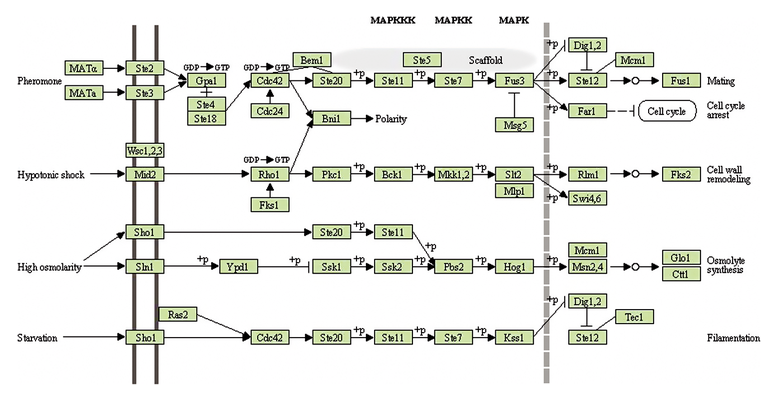
\includegraphics[width=0.8\textwidth]{./figs/494f01.eps}
    \caption{The yeast MAPK pathway from the KEGG database}
    \label{fig:MAPK}
\end{figure}

From the database we obtain $53$ markers which have been linked to MAPK signaling pathways biologically. 

After the above operations, we got the processed data with a $X\in\mathbb{R}^{112 \times 949} ,\, Y\in\mathbb{R}^{112 \times 53}$. 

Hereinafter, we denote $p$ as the number of explanatory variables, $q$ as the number of response variable, $n$ as the number of samples, $E$ as the random error matrix, and $B$ as the coefficient matrix, we can construct a multi-response linear model as following

\begin{equation}\label{eq:model}
    Y = XB + E. 
\end{equation}